\section{What is MPS?}
\label{section:MPS}

Language workbenches (LWB) are a tool to help language engineers create languages, particularly domain specific languages (DSL).
The term LWB was popularized in a 2005 article by Martin Fowler\cite{Fowler_lwb}.

Meta Programming System (MPS) is an opensource LWB that assists in the creation of Projectional languages.
It started in 2003 by JetBrains, and introduced to the world in Sergey Dmitriev's 2004 Paper ``Language Orientated Programming: the Next Programming Paradigm''\cite{dmitriev2004language}.

As discussed in section \ref{section:WhatIsPE}, When creating a projectional language one has to not only define the language but also how one interacts with it.
MPS lets you define languages and solutions in which you can use your defined language, in conjunction with languages defined by others, to write programs.

The following is an overview of how MPS implements the ideal of a projectional language, as well as the structure of this section: 

\begin{itemize}
    \item Abstract syntax
    \begin{itemize}
        \item Structure
        \item Behaviors
        \item Constraints
        \item Type system
    \end{itemize}
    \item Concrete syntax
    \begin{itemize}
        \item Editors
        \item Intentions
    \end{itemize}
    \item Generators
    \begin{itemize}
        \item Model-to-Model
        \item Model-to-Text
    \end{itemize}
\end{itemize}

MPS defines the different aspects of the language definitions with declarative DSLs, bundled together in what they call Aspects.

\subsection{Abstract Syntax: Structure}
Structure is what determines the abstract syntax of a language.
The most important item available in a Structure Aspect is the Concept.
Instances of concepts are called nodes and it is with these that the programmers construct their programs, i.e. their Abstract Syntax Trees (AST).

In principle a concept is a contains three types of things:
\begin{enumerate}
    \item properties: these primitives are integer, boolean, string, or enum items and could be seen as leaf values.
    \item children: these are other concepts, or collections of them, and could be seen as sub trees.
    \item references: these are relationships with other nodes in the AST. These turn the tree into a graph.
\end{enumerate}

Concepts follow some object orientated (OO) traits, such as being able to subtype, being abstract, and implementing interfaces.
At least one rootable concept needs to be defined in order to be able to create a program.

Other items available in the Structure Aspect are the Interface Concept, the Enumeration, the Constrained Data Type, and the Primitive Datatype.
\footnote{At time of writing we are unaware as to whether Data Type and Datatype are semantically different or if it is a style choice.}

Thus, the structure aspect defined how the AST can be structured.

Figure \ref{fig:concept_example} shows a concept with three children that implements two interfaces.

\begin{figure}[h]
    \centering
    \fbox{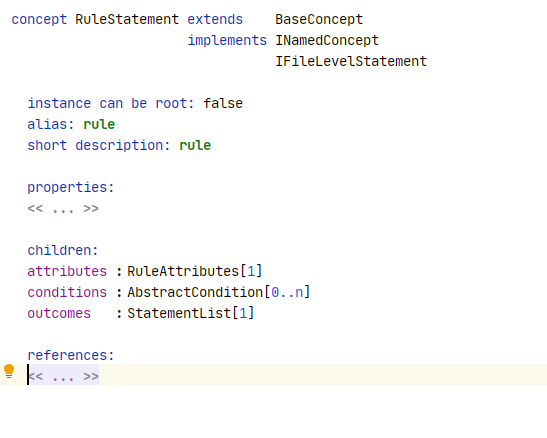
\includegraphics[width=0.75\textwidth]{Sections/images/concept_example.png}}
    \caption{Concept example}
    \label{fig:concept_example}
\end{figure}
 

\subsection{Abstract Syntax: Behaviors}
\emph{When referring to it's use in the MPS workbench, consistent with their use, we use the American spelling, Behavior.}
OO design usually bundles together data and methods that can act on that data.
Concepts are analogous to the data part of this equation.
Behavior fill the role of the methods in the OO analogy, defining the functionality that can be called on instantiated the nodes, as well as static methods which can be called on the Concept.
These methods include a constructor for a node.

The methods have public, private, or protected visibility.
If the Concept to which the behavior refers is abstract, the behavior itself can contain abstract Methods.
This allows a sort of polymorphism, as if a method is declared as being virtual then it will be called polymorphically.

Figure \ref{fig:behavior_example} show a constructor being added to a concept to initialize its children.
It has a method to allow other nodes to interrogate the condition of it having attributes.

\begin{figure}[h]
    \centering
    \fbox{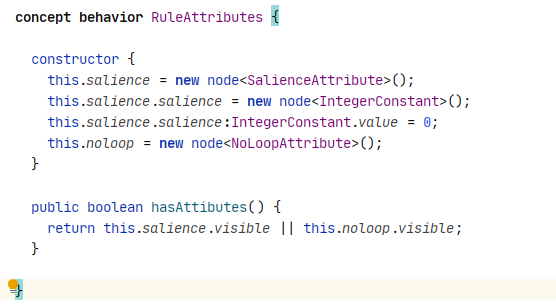
\includegraphics[width=0.75\textwidth]{Sections/images/behavior_example.png}}
    \caption{Behavior example}
    \label{fig:behavior_example}
\end{figure}
 

\subsection{Abstract Syntax: Constraints}
The constraints aspect adds further structural constraints to concepts.
These constraints are especially used to define scope.
Other constraints including allowing if a node can be a child, a parent, or an ancestor of this node.
the constraints aspect also allows preventing badly formed properties, children or references.

Figure \ref{fig:constraint_example} shows an example of a scope restraint that only allows local variables that are declared within the same rule or global variables declared in the same file.

\begin{figure}[h]
    \centering
    \fbox{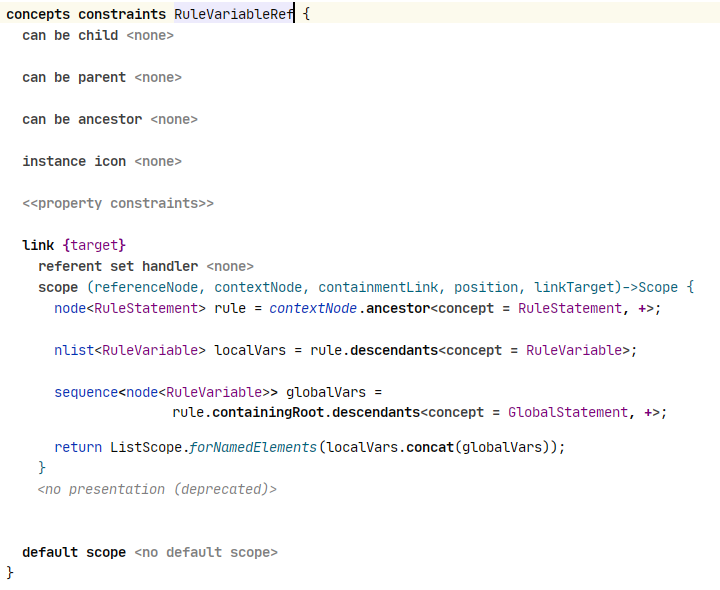
\includegraphics[width=0.95\textwidth]{Sections/images/constraint_example.png}}
    \caption{Constraint example}
    \label{fig:constraint_example}
\end{figure}
 

\subsection{Abstract Syntax: Type System}
The TypeSystem aspect and the constraints aspect together represent the static semantics of the language.
This aspect is for the computation and evaluation of types of variables, expressions and statements.

Rules that are available to calculate and enforce the type system include inference, subtyping, comparison and substitute type rules.

Figure \ref{fig:typesystem_example} shows an inference rule that is ensuring that the calculated type of the import statement matched the that of it's child called type.

\begin{figure}[h]
    \centering
    \fbox{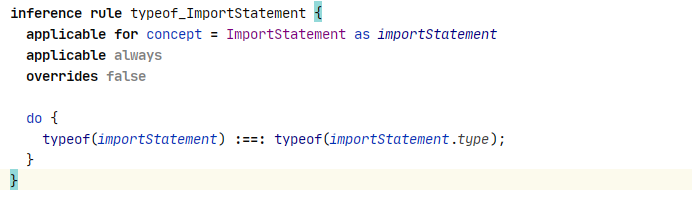
\includegraphics[width=0.75\textwidth]{Sections/images/typesystem_example.png}}
    \caption{Typesystem example}
    \label{fig:typesystem_example}
\end{figure}
 

\subsection{Concrete Syntax: Editors}
Editors define the notation of the nodes.
In effect it is the user interface of the language, how the AST is projected to the developer.
An editor is a swing panel that renders a tree of editor cells.
A concept can have multiple editors, thus offering multiple views on it.

The editor aspect is also where you can redefine what options will be presented to developers, through substitute menus.
Transformations can be defined, so that when a certain option is input by the developer, the existing AST is transformed to match the meaning of the choice.

Behavior of interactions can be defined, such as what will happen to the AST when a particular key press or editor action occurs at a particular location.

Figure \ref{fig:editor_example} shows a component with one projection for the concept shown in figure \ref{fig:concept_example}.
\begin{figure}[h]
    \centering
    \fbox{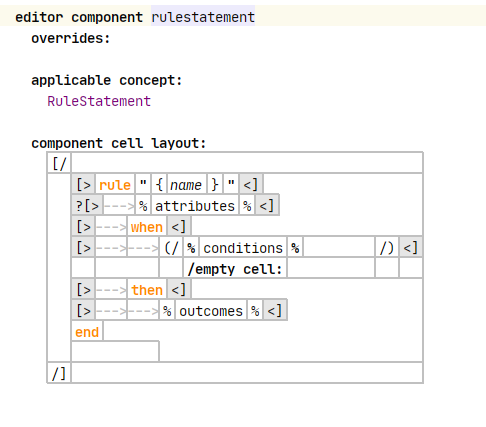
\includegraphics[width=0.65\textwidth]{Sections/images/editor_example.png}}
    \caption{Editor example}
    \label{fig:editor_example}
\end{figure}
 

\subsection{Concrete Syntax: Intentions}
In projectional editing it can be said that the IDE is a part of the concrete syntax.
Intentions make context aware suggestions for automatic changes to the program to the developer.

Figure \ref{fig:intention_example} shows an intention that allows the developer to add, remove or edit a property based on it's current value.
\begin{figure}[h]
    \centering
    \fbox{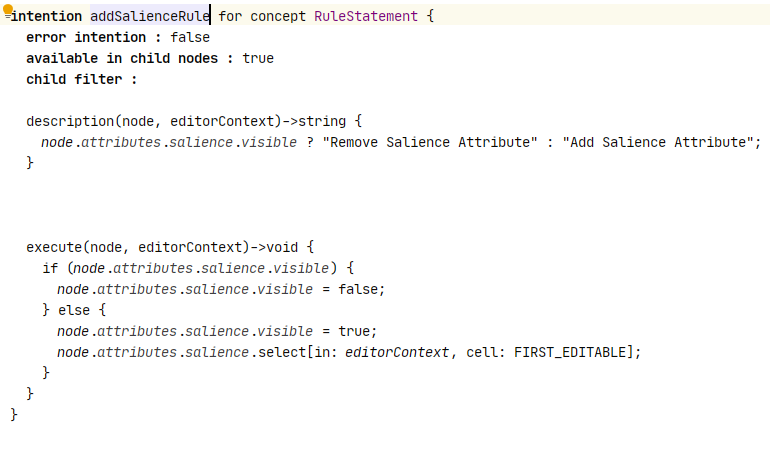
\includegraphics[width=0.75\textwidth]{Sections/images/intention_example.png}}
    \caption{Intention example}
    \label{fig:intention_example}
\end{figure}

\subsection{Generators: Model-to-Text}
Whilst designing a language is nice, it has to be able to do something, without doing so it has no semantic meaning.
It is possible to create interpreters that can use the AST generated by MPS.
However, the most common modality for MPS is to generate an output to be compiled and run by commonly known environments.
The output stage of generation is called TextGen.
It defined how a node will be turned into runnable code in plain text.

\subsection{Generators: Model-to-Model}
Whilst the base level languages will have text generation, most DSLs will perform model-to-model conversions.
These are known as Generator Aspects.
They transform code written in one language to another.
A concept can have multiple generators, aimed at different base level languages, such as Java (using MPS BaseLanguage), C (using mbeddr) or XML.